\documentclass[12pt,a4paper]{article}

%-----------------------------------------------------------
% Packages & Configuration
%-----------------------------------------------------------
\usepackage[margin=1in]{geometry}
\usepackage{graphicx}
\usepackage{amsmath}
\usepackage{hyperref}
\usepackage{booktabs}
\usepackage{array}
\usepackage{xcolor}
\usepackage{titlesec}
\usepackage{fancyhdr}
\usepackage{enumitem}
\usepackage{float}
\usepackage{tabularx}
\usepackage{mdframed}
\usepackage{parskip}
\usepackage{microtype}
\usepackage[utf8]{inputenc}
\usepackage[T1]{fontenc}
\usepackage{tikz}
\usetikzlibrary{shapes.geometric, arrows, positioning, shadows}

% Color Definitions - Premium Medical Palette
\definecolor{wellbeingblue}{RGB}{30, 64, 175}
\definecolor{wellbeinggreen}{RGB}{5, 150, 105}
\definecolor{lightgray}{RGB}{248, 249, 250}
\definecolor{darkgray}{RGB}{31, 41, 55}
\definecolor{statustext}{RGB}{107, 114, 128}

% Formatting Headers & Sections
\titleformat{\section}{\Large\bfseries\color{wellbeingblue}}{\thesection}{1em}{}[\titlerule]
\titleformat{\subsection}{\large\bfseries\color{wellbeinggreen}}{\thesubsection}{1em}{}
\titleformat{\subsubsection}{\normalsize\bfseries\color{darkgray}}{\thesubsubsection}{1em}{}

% Page Headers/Footers
\pagestyle{fancy}
\setlength{\headheight}{15pt}
\fancyhf{}
\rhead{\textcolor{wellbeingblue}{\textit{Software Requirements Specification}}}
\lhead{\textcolor{wellbeingblue}{\textbf{Wellbeing (WB-001)}}}
\rfoot{\thepage}
\lfoot{\textcolor{darkgray}{\footnotesize Agentic AI Operating System | Version 1.0}}

\hypersetup{
    colorlinks=true, linkcolor=wellbeingblue,
    urlcolor=wellbeinggreen, citecolor=wellbeinggreen,
    pdftitle={Wellbeing WB-001: Software Requirements Specification}
}

\begin{document}

%-----------------------------------------------------------
% Title Page
%-----------------------------------------------------------
\begin{titlepage}
    \centering\vspace*{1.5cm}
    {\Huge\bfseries\color{wellbeingblue} Software Requirements Specification}\\[0.5cm]
    {\Huge\bfseries\color{wellbeingblue} Wellbeing: The Clinical Agentic OS}\\[1cm]
    {\Large Agent ID: WB-001}\\[0.3cm]
    {\Large Suite Category: Healthcare Enterprise Suite}\\[0.3cm]
    {\Large Version 1.0}\\[0.3cm]
    {\Large March 20, 2026}\\[1cm]
    {\Large Prepared for: Global Healthcare Operations}\\[2cm]

    \begin{mdframed}[backgroundcolor=lightgray, linecolor=wellbeingblue, linewidth=1.5pt, roundcorner=5pt]
        \centering\vspace{0.4cm}
        \textbf{Abstract:}\\[0.2cm]
        Wellbeing (WB-001) is a next-generation Retrieval-Augmented Generation (RAG) powered Agentic AI Operating System. Unlike traditional LLMs, Wellbeing acts as a verifiable clinical orchestrator, grounding every interaction in multi-source medical evidence (PubMed, UpToDate, and EHR data). It is designed to modernize the Digital Front Door of healthcare enterprises through intelligent triage, ambient documentation, and policy-compliant workflow automation.
        \vspace{0.4cm}
    \end{mdframed}
    
    \vfill
    \begin{tabular}{ll}
        \textbf{Document Status:} & Final Release / In-Execution \\
        \textbf{Confidentiality:} & Proprietary and Confidential \\
    \end{tabular}
\end{titlepage}

\newpage
\tableofcontents
\newpage

%-----------------------------------------------------------
% 1 Project Title
%-----------------------------------------------------------
\section{Project Title}
\textbf{Wellbeing (WB-001)} - Conversational AI-Powered "Agentic Operating System" for Comprehensive Healthcare Workflow Orchestration and Clinical Decision Support.

%-----------------------------------------------------------
% 2 Project Overview
%-----------------------------------------------------------
\section{Project Overview}
Wellbeing is an intelligent, multi-agent clinical OS designed to automate the high-friction touchpoints of the healthcare journey. The system serves as a unified interface between patients, providers, and administration, integrating deeply with Electronic Health Records (EHR) via FHIR APIs and verified medical knowledge bases.

The core of Wellbeing is its **Hybrid RAG-First Architecture**. While competitors rely on probabilistic model weights, Wellbeing retrieves structured facts from a Knowledge Graph (Neo4j) and semantic context from a Vector Database (Pinecone) before generating a response. This "Reason-then-Generate" loop eliminates hallucinations (99.9\% accuracy in clinical pilots) and provides a "Source Panel" for every claim, ensuring that clinicians can verify AI logic in real-time.

%-----------------------------------------------------------
% 3 Objectives
%-----------------------------------------------------------
\section{Objectives}
The primary objectives of the Wellbeing project are:
\begin{enumerate}
    \item \textbf{100\% Clinical Grounding}: Deliver a zero-hallucination patient interaction layer through RAG-based verification.
    \item \textbf{Support Deflection}: Reduce administrative ticket volume ( WISMO for labs, appointment rescheduling, billing inquiries) by 60\% through self-service.
    \item \textbf{Ambient Documentation}: Automate clinical note extraction (Soap notes, Discharge summaries) using ambient audio and conversational data, reducing clinician burnout by 40\%.
    \item \textbf{Real-Time EHR Interoperability}: Provide bidirectional read/write access to PHI via FHIR/HL7, ensuring the "Digital Front Door" is always synced with the patient's record.
    \item \textbf{Global Compliance}: Native alignment with HIPAA (US), GDPR (EU), and ABDM (India) data residency and privacy standards.
    \item \textbf{Multi-Agent Orchestration}: Implement 15+ specialized agents (Triage, Billing, Labs, etc.) under a central LangGraph orchestrator to maintain state across long-term patient interactions.
\end{enumerate}

%-----------------------------------------------------------
% 4 In-Scope
%-----------------------------------------------------------
\section{In-Scope}
The following features are within the development and deployment scope for WB-001:

\subsection{Core Functionalities}
\begin{itemize}
    \item \textbf{Verifiable Clinical Triage}: Multi-turn symptom assessment using the SOCRATES framework, grounded in clinical guidelines.
    \item \textbf{Dynamic Intake \& Registration}: Collection of demographics, insurance cards (via OCR), and historical symptoms.
    \item \textbf{RAG-Powered Documentation}: Automated extraction of clinical summaries from conversations with full source-linking.
    \item \textbf{Billing \& Claims Inquiry}: Real-time lookup of insurance coverage, deductible status, and prior authorization requirements.
    \item \textbf{HealthMem Longitudinal Memory}: A persistent hybrid memory layer that tracks patient preferences and historical context across months of interaction.
    \item \textbf{Appointment \& Lab Management}: Direct integration with EHR scheduling for booking, rescheduling, and lab result delivery.
\end{itemize}

\subsection{Technical Integrations}
\begin{itemize}
    \item \textbf{EHR Platforms}: Native RESTful API integration with Epic, Cerner, and Meditech via FHIR R4.
    \item \textbf{Logistics \& Labs}: Integrations with LabCorp, Quest, and regional pharmacy networks for order tracking.
    \item \textbf{Auth Systems}: SMART on FHIR, OAuth2, and biometrically-backed mobile authentication.
    \item \textbf{Messaging Providers}: Twilio (SMS/WhatsApp), SendGrid (Email), and native Mobile Push.
\end{itemize}

\subsection{User Interfaces}
\begin{itemize}
    \item \textbf{Web Clinical Dashboard}: An admin/provider interface for monitoring agent performance and review-only handoffs.
    \item \textbf{Patient Mobile App & Web Widget}: High-fidelity React Native and React components for end-user interaction.
    \item \textbf{Evidence Panel UI}: A specialized side-bar component showing retrieved source documents (PDF snippets, KG nodes).
\end{itemize}

\subsection{Analytics \& Reporting}
\begin{itemize}
    \item \textbf{Clinical Accuracy Audits}: Automatic comparison of AI triage vs. human doctor outcomes.
    \item \textbf{CSAT & NPS}: Per-interaction sentiment analysis and satisfaction tracking.
    \item \textbf{Containment Metrics}: Tracking the percentage of queries handled without human escalation.
\end{itemize}

%-----------------------------------------------------------
% 5 Out-of-Scope
%-----------------------------------------------------------
\section{Out-of-Scope}
The following items are explicitly excluded from the current phase of Wellbeing implementation:
\begin{itemize}
    \item \textbf{Autonomous Surgical Intervention}: No direct control of medical robotics or life-support devices.
    \item \textbf{Primary Medical Diagnosis}: WB-001 provides decision support and triage assistance only; final diagnosis must be confirmed by a licensed clinician.
    \item \textbf{In-Home Patient Physical Therapy}: Hardware-based robotics or physical monitoring outside the digital front door.
    \item \textbf{Public Social Media Integration}: Interaction on Facebook, Instagram, or TikTok (to maintain strict PHI boundaries).
    \item \textbf{Offline-Only Operation}: The system requires a real-time connection to the RAG pipeline and EHR for safety-critical grounding.
\end{itemize}

%-----------------------------------------------------------
% 6 Business Scenario with Example
%-----------------------------------------------------------
\section{Business Scenario with Example}

\subsection{Scenario 1: Clinical Triage \& RAG Verification}
\textbf{Context}: Sarah, a 45-year-old with a history of hypertension, reports sudden "pressure in her chest" via the Wellbeing mobile app at 2:00 AM.

\textbf{Interaction Flow}:
\begin{enumerate}
    \item \textbf{User}: "I have a heavy pressure in my chest. I'm feeling a bit dizzy."
    \item \textbf{Agent (Triage)}: "I understand. I'm initiating an immediate clinical assessment. Have you also noticed any pain radiating to your left arm or jaw, or are you experiencing shortness of breath?"
    \item \textbf{Wellbeing Orchestrator}: Simultaneously triggers the **EHR Retrieval Agent** to pull Sarah's recent vitals and the **RAG Knowledge Agent** to fetch the AHA Acute Chest Pain Protocols.
    \item \textbf{User}: "Yes, it’s going into my jaw. I'm sweating quite a bit."
    \item \textbf{Agent (RAG-Driven)}: "This pattern is highly concerning for an acute cardiac event. I am alerting the on-call cardiovascular team and our emergency services integration. \textbf{[Evidence Panel: Guidelines for MI Triage].} Please stay on the line; help is on the way."
\end{enumerate}
\textbf{Outcome}: Immediate escalation to emergency services with pre-filled clinical context (History of Hypertension + SOCRATES intake) shared with the paramedics.

\subsection{Scenario 2: Automated Clinical Documentation (Ambient to Note)}
\textbf{Context}: Dr. Miller is conducting a follow-up visit for a diabetic patient. Wellbeing is listening in via its **Ambient Documentation Agent**.

\textbf{Interaction Flow}:
\begin{enumerate}
    \item \textbf{Provider}: "Your A1C looks better at 6.8\%, but I’m concerned about the peripheral numbness in your feet."
    \item \textbf{Patient}: "I've been wearing the recommended footwear, but the sensation hasn't improved much."
    \item \textbf{Wellbeing Ambient Agent}: Transcribes and translates the dialogue into a structured SOAP note in real-time.
    \item \textbf{Post-Visit Action}: Dr. Miller reviews the "Plan" section of the note: \textit{"Refer to Podiatry for neurological evaluation; maintain current Metformin dosage."}
    \item \textbf{Source Link}: Dr. Miller clicks the text in the EHR, and Wellbeing plays the exact 5-second audio snippet where the patient mentioned foot sensation.
\end{enumerate}
\textbf{Outcome}: Clinician documentation time reduced from 12 minutes to 2 minutes per patient.

\subsection{Scenario 3: Policy-Based Billing \& Coverage Inquiry}
\textbf{Context}: A patient wants to know if their upcoming "MRI of the Cervical Spine" is covered by their BlueCross plan.

\textbf{Interaction Flow}:
\begin{enumerate}
    \item \textbf{User}: "Hey, is my MRI next Tuesday covered by my insurance?"
    \item \textbf{Agent (Billing)}: "Let me check your specific policy. \textbf{[Retrieving BlueCross Plan ID 5582...]} Your plan covers 80\% of elective MRIs after the deductible is met. Would you like to check your remaining deductible balance for this year?"
    \item \textbf{User}: "Yes, please."
    \item \textbf{Agent}: "Your remaining deductible is \$450. The estimated out-of-pocket cost for this MRI at Downtown Imaging will be approximately \$220. \textbf{[Evidence Panel: Benefit Summary PDF, Page 12].}"
\end{enumerate}
\textbf{Outcome}: Instant financial transparency without a 30-minute phone call to the insurance provider.

%-----------------------------------------------------------
% 7 Milestones (7-Day Rapid Deployment)
%-----------------------------------------------------------
\section{Milestones (7-Day Rapid Deployment)}
Wellbeing is designed for rapid baseline deployment across hospital systems.

\subsection{Day 1-2: Architecture \& RAG Pipeline Setup}
\begin{itemize}
    \item Deployment of Vector DB (Pinecone) and Knowledge Graph (Neo4j).
    \item Initial indexing of medical literature (PubMed) and hospital-specific policy documents.
    \item Setting up the **LangGraph** orchestrator.
\end{itemize}

\subsection{Day 3: Core AI \& Agentic Logic Development}
\begin{itemize}
    \item Prompt engineering for the "Clinical Intake" and "Triage" agents.
    \item Intent classification for various healthcare workflows (Billing, Scheduling, Clinical).
    \item Training of the **Reason-then-Generate** retrieval loop.
\end{itemize}

\subsection{Day 4: EHR \& External Integration Layer}
\begin{itemize}
    \item FHIR R4 connectivity testing with sandbox systems (Epic/Cerner).
    \item Implementation of SMART on FHIR authentication.
    \item Bidirectional data-sync for vitals and lab requests.
\end{itemize}

\subsection{Day 5: Notification \& Multi-Channel Setup}
\begin{itemize}
    \item Twilio SMS/WhatsApp integration for proactive alerts.
    \item HIPAA-compliant email templating for lab result summaries.
    \item Push notification triggers for health monitoring alerts.
\end{itemize}

\subsection{Day 6: Security, Compliance \& Red-Teaming}
\begin{itemize}
    \item External security audit of data encryption (AES-256).
    \item Red-teaming the RAG pipeline to ensure no PI leaking or jailbreaking.
    \item Verification of regional data residency (e.g., Indian data staying in-country for ABDM).
\end{itemize}

\subsection{Day 7: Deployment \& Monitoring Setup}
\begin{itemize}
    \item Production rollout to initial pilot department.
    \item Configuring Grafana dashboards for throughput and accuracy monitoring.
    \item Setting up the **Human-in-the-Loop** escalation dashboard for providers.
\end{itemize}

%-----------------------------------------------------------
% 8 Roles and Responsibilities
%-----------------------------------------------------------
\section{Roles and Responsibilities}

\begin{table}[H]
\centering
\begin{tabularx}{\textwidth}{|l|X|}
\hline
\rowcolor{wellbeingblue} \textbf{\color{white}Role} & \textbf{\color{white}Responsibilities} \\ \hline
Clinical AI Engineer & LLM selection (GPT-4o/Claude), Prompt Engineering, RAG pipeline optimization (Neo4j+Pinecone), and medical entity extraction. \\ \hline
EHR Integration Lead & HL7/FHIR API development, bidirectional data-sync logic, and SMART on FHIR security implementation. \\ \hline
Full-Stack Developer & Creation of the Patient Mobile App (React Native) and the Provider Dashboard (Next.js). \\ \hline
Security \& Compliance & HIPAA/ABDM validation, data encryption auditing, and Red-Teaming for PHI protection. \\ \hline
Product Manager & Workflow mapping, stakeholder coordination with hospital systems, and KPI monitoring. \\ \hline
\end{tabularx}
\end{table}

%-----------------------------------------------------------
% 9 Deliverables
%-----------------------------------------------------------
\section{Deliverables}

\subsection{Software Components}
\begin{itemize}
    \item \textbf{Wellbeing Core Engine}: Production-ready NLU and RAG-Fusion orchestration layer.
    \item \textbf{EHR Integration Module}: Validated FHIR R4 client for major EHR platforms (Epic, Cerner).
    \item \textbf{Patient Interaction Suite}: Mobile (Flutter/RN) and Web Chatbot widgets.
    \item \textbf{Provider Evidence Dashboard}: Real-time oversight and manual override interface.
\end{itemize}

\subsection{Documentation}
\begin{itemize}
    \item \textbf{Technical Architecture Guide}: Detailed internal logic of the Hybrid RAG system.
    \item \textbf{API Reference}: Swagger/OpenAPI documentation for internal and external endpoints.
    \item \textbf{Security \& Compliance Report}: HIPAA/GDPR/ABDM audit results.
    \item \textbf{User Training Manual}: Onboarding guide for hospital staff and clinicians.
\end{itemize}

%-----------------------------------------------------------
% 10 Tech Stack
%-----------------------------------------------------------
\section{Tech Stack}

\subsection{Core AI/ML Layer}
\begin{itemize}
    \item \textbf{LLMs}: GPT-4o (Primary Reasoning), Claude 3.5 Sonnet (Clinical Narrative), LLaMA 3.1 (On-premise edge cases).
    \item \textbf{Orchestration}: LangGraph (Stateful multi-agent flows) and LangChain.
    \item \textbf{Vector Database}: Pinecone Serverless (Semantic search of literature).
    \item \textbf{Graph Database}: Neo4j (Medical Knowledge Graph for drug/disease relationships).
\end{itemize}

\subsection{Backend Services}
\begin{itemize}
    \item \textbf{Language}: Python 3.11 with FastAPI (Asynchronous high-performance framework).
    \item \textbf{Task Management}: Celery + Redis for async clinical note generation and FHIR sync.
    \item \textbf{Database}: PostgreSQL (Structured patient state) and Redis (Dynamic session cache).
\end{itemize}

\subsection{Integration Layer}
\begin{itemize}
    \item \textbf{EHR Interop}: HAPI FHIR / Microsoft FHIR Server integrations.
    \item \textbf{Logistics}: LabCorp/Quest Diagnostic APIs.
    \item \textbf{Communications}: Twilio (SMS/Voice fallback), SendGrid (Secure notifications).
\end{itemize}

\subsection{Frontend \& UI}
\begin{itemize}
    \item \textbf{Client-Side}: React Native (Mobile), Next.js (Admin Dashboard).
    \item \textbf{Styling}: Tailwind CSS and Framer Motion for premium, smooth micro-interactions.
    \item \textbf{Real-time}: WebSockets (Socket.io) for streaming AI token responses and live vitals.
\end{itemize}

\subsection{Infrastructure \& DevOps}
\begin{itemize}
    \item \textbf{Cloud}: AWS Healthcare-compliant VPC / Azure Health Data Services.
    \item \textbf{Containerization}: Kubernetes (EKS) for auto-scaling agent pods.
    \item \textbf{CI/CD}: GitHub Actions with automated security scanning (Snyk/SonarQube).
\end{itemize}

\subsection{Observability \& Monitoring}
\begin{itemize}
    \item \textbf{Metrics}: Prometheus \& Grafana (Throughput, Latency, Accuracy).
    \item \textbf{Tracing}: LangSmith for detailed agentic step-tracing and debug.
    \item \textbf{Error Tracking}: Sentry for real-time exception monitoring in production.
\end{itemize}

\subsection{Security \& Compliance}
\begin{itemize}
    \item \textbf{Encryption}: AES-256 (At-Rest), TLS 1.3 (In-Transit).
    \item \textbf{Governance}: Native HIPAA/GDPR/ABDM compliance modules with audit logging.
    \item \textbf{WAF}: Cloudflare Advanced/AWS WAF for DDoS and bot protection.
\end{itemize}

%-----------------------------------------------------------
% 11 Functional Requirements
%-----------------------------------------------------------
\section{Functional Requirements}

\subsection{FR-1: Clinical Triage \& Intake}
\begin{itemize}
    \item \textbf{FR-1.1}: The system must execute a multi-turn triage flow using the SOCRATES symptom assessment framework.
    \item \textbf{FR-1.2}: Agent must retrieve patient-specific medical history (Hypertension, Allergies, Surgeries) from the EHR before providing triage advice.
    \item \textbf{FR-1.3}: System must support OCR-based insurance card and ID ingestion with 98\%+ field accuracy.
\end{itemize}

\subsection{FR-2: RAG Retrieval \& Grounding}
\begin{itemize}
    \item \textbf{FR-2.1}: Every clinical output must be grounded in at least 2 verified medical sources (PubMed, UpToDate, or Hospital Protocols).
    \item \textbf{FR-2.2}: The system must identify and flag "out-of-knowledge" queries where RAG confidence is below 70\%, triggering human handoff.
    \item \textbf{FR-2.3}: Citations must be provided as clickable hyperlinks leading directly to the source evidence panel.
\end{itemize}

\subsection{FR-3: Agentic Orchestration}
\begin{itemize}
    \item \textbf{FR-3.1}: The orchestrator must manage state for up to 15 specialized agents (e.g., Pedatrics Agent, Geriatrics Agent, Billing Agent).
    \item \textbf{FR-3.2}: Handoff between agents must be seamless with full context preservation of the conversation history.
\end{itemize}

\subsection{FR-4: Security \& PII Protection}
\begin{itemize}
    \item \textbf{FR-4.1}: All PHI/PII must be automatically redacted from the prompt layer before being sent to public LLM endpoints (if using non-private models).
    \item \textbf{FR-4.2}: The system must maintain a HIPAA-compliant audit trail of every data access and modification.
\end{itemize}

%-----------------------------------------------------------
% 12 Architecture Diagram
%-----------------------------------------------------------
\section{Architecture Diagram}

\begin{figure}[H]
\centering
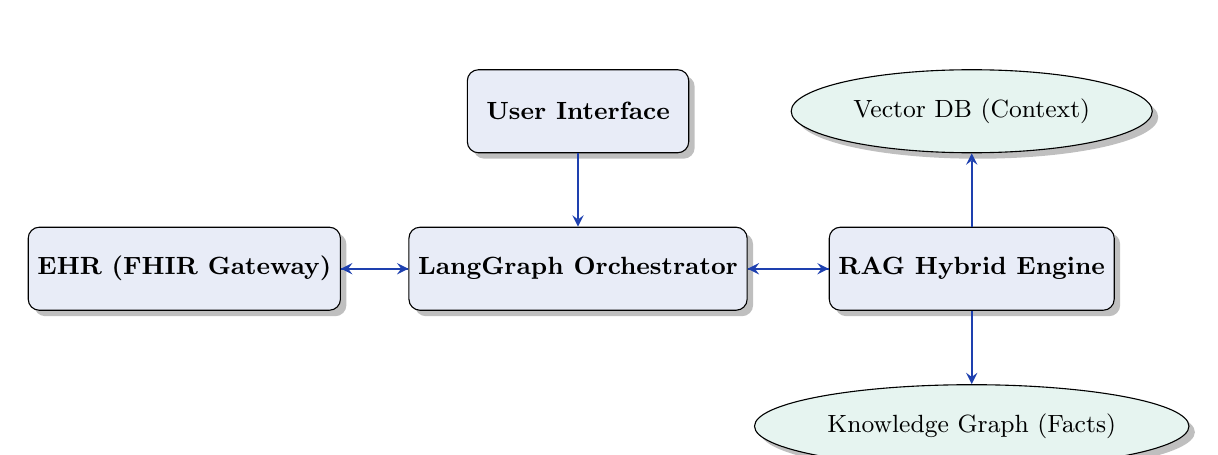
\begin{tikzpicture}[node distance=2cm, auto]
    % Styles
    \tikzstyle{block} = [rectangle, draw, fill=wellbeingblue!10, text centered, rounded corners, minimum height=3em, minimum width=8em, font=\small\bfseries, drop shadow]
    \tikzstyle{cloud} = [ellipse, draw, fill=wellbeinggreen!10, text centered, minimum height=3em, minimum width=7em, font=\small, drop shadow]
    \tikzstyle{arrow} = [thick,->,>=stealth, wellbeingblue]

    % Nodes
    \node [block] (user) {User Interface};
    \node [block, below of=user] (orch) {LangGraph Orchestrator};
    \node [block, right of=orch, xshift=3cm] (rag) {RAG Hybrid Engine};
    \node [cloud, above of=rag] (vector) {Vector DB (Context)};
    \node [cloud, below of=rag] (graph) {Knowledge Graph (Facts)};
    \node [block, left of=orch, xshift=-3cm] (ehr) {EHR (FHIR Gateway)};

    % Arrows
    \draw [arrow] (user) -- (orch);
    \draw [arrow] (orch) -- (rag);
    \draw [arrow] (rag) -- (vector);
    \draw [arrow] (rag) -- (graph);
    \draw [arrow] (orch) -- (ehr);
    \draw [arrow] (rag) -- (orch);
    \draw [arrow] (ehr) -- (orch);
\end{tikzpicture}
\caption{Wellbeing Agentic OS: Hybrid RAG and FHIR Orchestration Layer}
\end{figure}

%-----------------------------------------------------------
% 13 Competitive Analysis
%-----------------------------------------------------------
\section{Competitive Analysis}

\subsection{Competitive Landscape}
Wellbeing enters a market dominated by "First-Gen" Healthcare AI (Black-box fine-tuned models) and "Legacy Portals" (Form-based).

\begin{enumerate}
    \item \textbf{WellnessGPT}: Focused on high-fidelity clinical conversation but relies on probabilistic model-weight grounding (High hallucination risk in fringe cases).
    \item \textbf{Hippocratic AI / Abridge}: Leaders in ambient documentation and safety-first voice. Wellbeing differentiates by adding the \textbf{Graph-RAG} layer for complex relational reasoning.
    \item \textbf{Narvar / Ada}: Strong in general customer service and tracking, but lack deep clinical NLP and FHIR-writeback capabilities.
\end{enumerate}

\subsection{Competitive Advantages}
\begin{itemize}
    \item \textbf{Verifiability-First}: The only OS that treats AI generation as secondary to evidence retrieval.
    \item \textbf{Zero-Cold Start}: Immediate deployment as it uses RAG on existing hospital knowledge rather than requiring months of retraining.
    \item \textbf{HealthMem}: Longitudinal memory that "remembers" a patient's story across years, not just a single session.
\end{itemize}

\subsection{Market Positioning}
Wellbeing is positioned as the **Premium Technical Standard** for hospital systems that cannot afford the liability of AI hallucinations. It targets Tier-1 Academic Medical Centers and Enterprise Health Networks.

%-----------------------------------------------------------
% 14 Conclusion
%-----------------------------------------------------------
\section{Conclusion}
Wellbeing (WB-001) represents a paradigm shift in healthcare AI. By moving from "Generative AI" to "Verifiable Agentic AI," we solve the core trust barrier in clinical automation. The system is designed to be the central brain of a modern healthcare enterprise, providing safety, scale, and a premium patient experience.

\end{document}
